\documentclass{beamer}
\usepackage{beamerthemesplit}
\usepackage{color,colortbl}
\usepackage{amsfonts}
\usepackage{multimedia}
\usepackage{animate}
\usepackage{wrapfig}
\usepackage{multicol}
%\setlength{\textwidth}{15cm}           %Sets the width of the printable area of the page to 15cm
%\setlength{\topmargin}{0cm}            %Space from the toprule to the top of the text (first line) to 0 cm.
%\setlength{\footskip}{0cm}               %Space from the bottom of the text to the footnote (or footrule) to 0 cm.
\setlength{\marginparwidth}{0cm}   
\setlength{\columnsep}{0cm}
\setbeamertemplate{caption}{\insertcaption} 

\definecolor{cvggreen}{RGB}{4,71,79}
\definecolor{LRed}{rgb}{1,.8,.8}


\mode<presentation>
{
%Darmstadt
\usetheme[]{Amsterdam}
}
\title{Marchiatura digitale di sequenze video stereoscopiche a disparit\`{a} coerente}
\author{Benedetta Barbetti\\ 
		Michaela Servi}
\institute{Universit\`{a} degli studi di Firenze}
\date{10 Dicembre 2015}


\begin{document}

\begin{frame}
\titlepage
\end{frame}

\begin{section}{Introduzione}
\subsection{Video Stereoscopici}

\begin{frame}[t]{\textsc{Contesto}}
Numerose applicazioni di elaborazione di immagini e video richiedono esplicite informazioni sulla \textbf{profondit\`{a}} della scena:
\setlength{\columnsep}{0cm}
\begin{columns}
\begin{column}{4cm}
\begin{center}
\setbeamertemplate{blocks}[rounded][shadow=false]
	\setbeamercolor{block body}{use=structure,fg=black,bg=lightgray} 	
\begin{block}{Campi applicativi}
		\begin{itemize}
			\item \small{Medicina} 
			\item Robotica
			\item Tracking
			\item Industria manifatturiera
			\item Cinema
		\end{itemize}	
	\end{block}
	
%	\textbf{Caratteristiche}:
%			\vspace*{0.5em}
%			%\begin{small}
%			\begin{itemize}
%			\item \small{Medicina} 
%			\item Robotica
%			\item Tracking
%			\item Industria manifetturiera
%			\item Cinema
%			\end{itemize}
%			%\end{small}

\end{center}
\end{column}
\begin{column}{6cm}
\begin{figure}
\centering
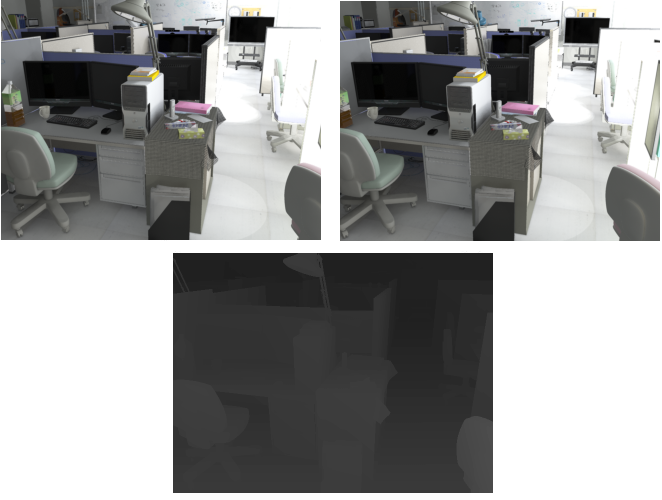
\includegraphics[width=1\linewidth]{./img/track.png}
\end{figure}
\end{column}
\end{columns}
\end{frame}


\begin{frame}[t]{\textsc{Video Stereoscopici}}
	\setbeamertemplate{blocks}[rounded][shadow=false]
	\setbeamercolor{block title}{use=structure,fg=black,bg=lightgray} 
	\setbeamercolor{block body}{use=structure,fg=black,bg=lightgray} 	
\begin{block}
	\center{Il \textbf{video stereoscopico} \`{e} ottenuto da due riprese con una \textbf{coppia di telecamere} adiacenti successivamente sovrapposte}
\end{block}
	\vspace{1em}
\begin{center}
\movie[width=8cm,height=5cm,autostart,loop,poster]{}{./img/alice.mp4}
\end{center}
\end{frame}





\begin{frame}[t]{\textsc{Dispositivi di ripresa e visualizzazione}}
\begin{columns}
\begin{column}{5cm}
\begin{center}
\setbeamertemplate{blocks}[rounded][shadow=false]
	\setbeamercolor{block body}{use=structure,fg=black,bg=lightgray} 
	\setbeamerfont{block body}{size=\tiny}	
\begin{block}{Sistema di ripresa stereo}
		\begin{itemize}
			\item  \small{Due telecamere sincronizzate
			\item Correttamente allineate
			\item Stessa calibrazione}
		\end{itemize}	
	\end{block}
\end{center}
\centering
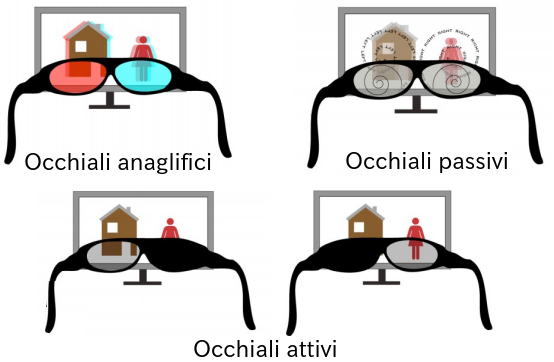
\includegraphics[width=1\linewidth]{./img/display.png}
\end{column}

\begin{column}{5cm}

\centering
\vspace{0.7em}
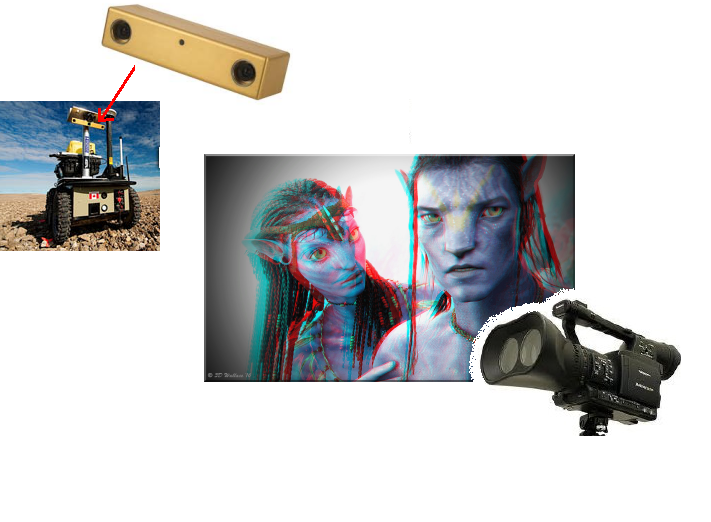
\includegraphics[width=1\linewidth]{./img/camere.png}
\vspace{-2.8em}
\begin{center}
\setbeamertemplate{blocks}[rounded][shadow=false]
	\setbeamercolor{block body}{use=structure,fg=black,bg=lightgray} 		
\begin{block}{Sistema di riproduzione}
		\begin{itemize}
			\item  \small{Attivo: lenti sincronizzate con il televisore
			\item Passivo: lenti diversamente polarizzate
			\item Anaglifico: lenti passive con filtri di colore diverso}
		\end{itemize}	
	\end{block}
\end{center}
\end{column}
\end{columns}
\end{frame}








\begin{frame}[t]{\textsc{Necessit\`{a} di una marchiatura}}
	\setbeamertemplate{blocks}[rounded][shadow=false]
	\setbeamercolor{block body}{use=structure,fg=black,bg=lightgray} 	
\begin{center}
\begin{block}{Precedenti motivazioni}
\begin{itemize}
\item  Sicurezza
\item  Copyright
\end{itemize}
\end{block}
\vspace{1em}
\begin{block}{Nuove motivazioni}
\begin{itemize}
\item Poco nello stato dell'arte
\item Migliorare la qualit\`{a} visiva dei contenuti marchiati utilizzando la particolarit\`{a} dei contenuti 3D
\end{itemize}
\end{block}
\end{center}
\end{frame}


\begin{frame}[t]{\textsc{Scopo di questa tesi}}


\end{frame}

\end{section}

\begin{section}{Stereoscopia}
\subsection{Principi della stereoscopia}
\begin{frame}[t]{\textsc{Stereoscopia}}
\vspace{-1em}
\begin{center}
	\setbeamertemplate{blocks}[rounded][shadow=false]
	\setbeamercolor{block title}{use=structure,fg=black,bg=lightgray} 
	\setbeamercolor{block body}{use=structure,fg=black,bg=lightgray} 		
\begin{block}{}
	\center Tecnica di realizzazione e visione di immagini e filmati, atta a trasmettere una illusione di \textbf{tridimensionalit\`{a}}, analoga a quella generata dalla visione binoculare del sistema visivo umano
	\end{block}
\end{center}
\begin{center}
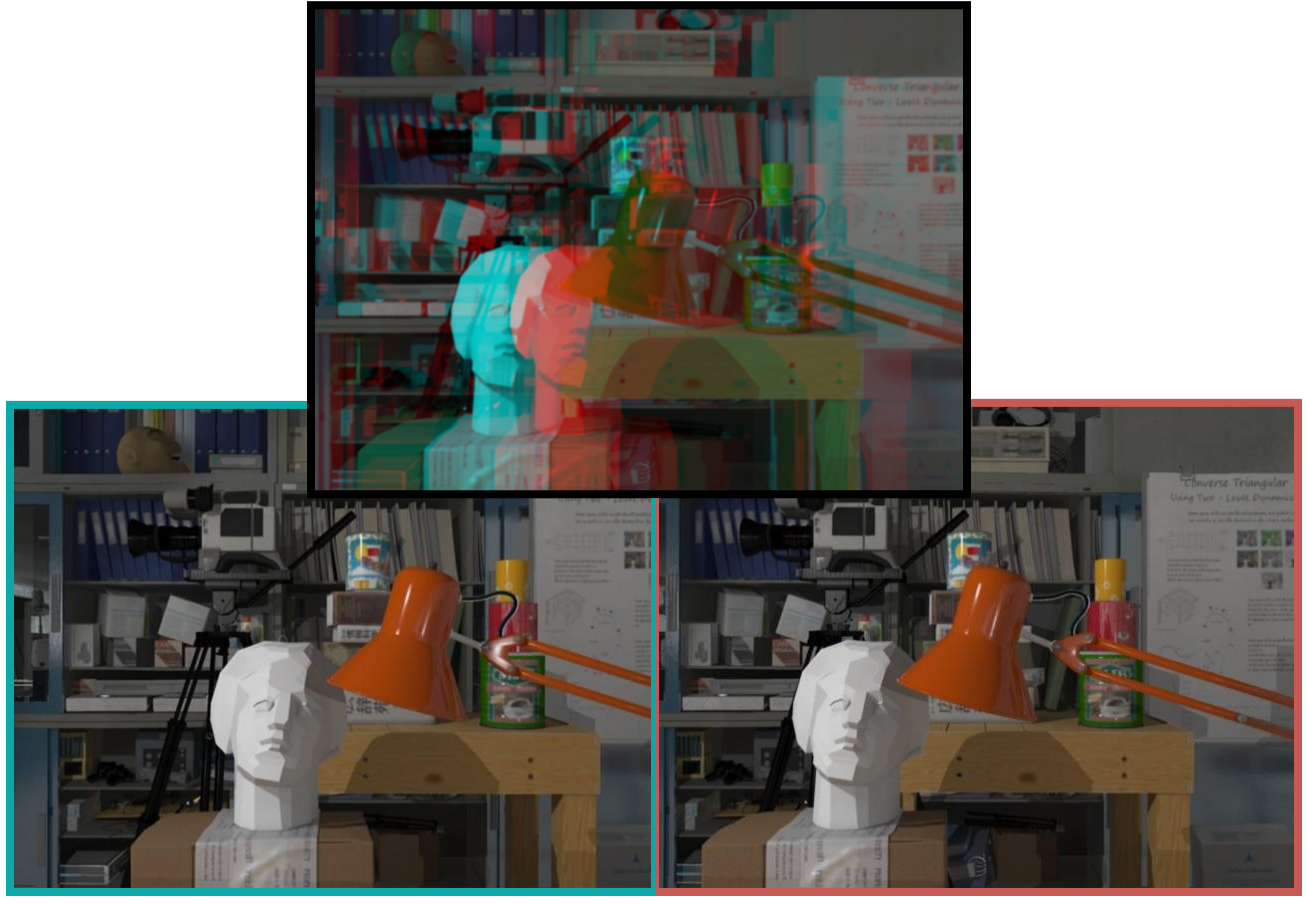
\includegraphics[width=0.7\linewidth]{./img/stereo.png}
\end{center}
\end{frame}

\begin{frame}[t]{\textsc{Background}}

\begin{columns}
\begin{column}{5cm}
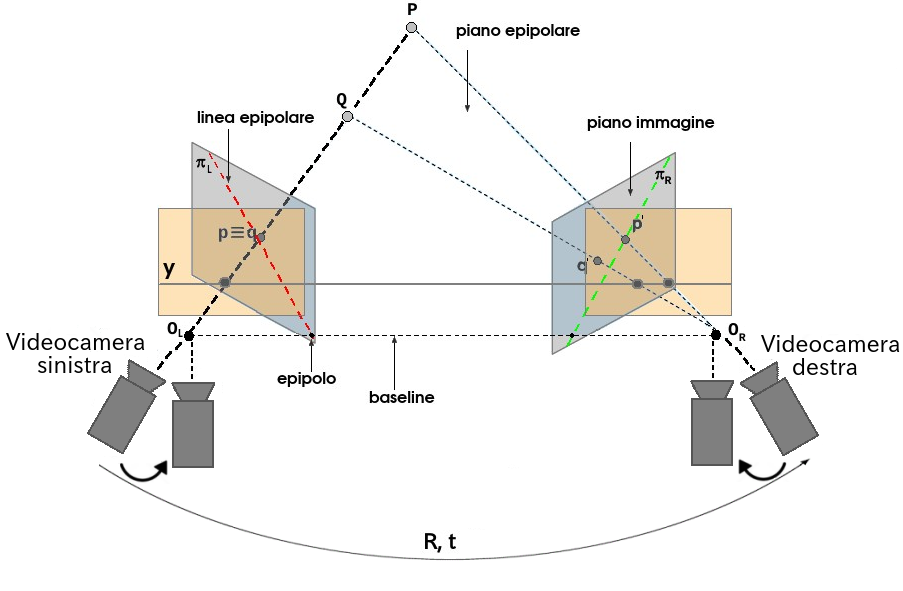
\includegraphics[width=1.1\linewidth]{./img/rect.png}

\begin{itemize}
\item[1.] \small{Calibrazione parametri interni ed esterni
\item[2.] Rettificazione
\item[3.] Calcolo delle corrispondenze
\item[4.] Computazione mappa di disparit\`{a}}
\end{itemize}

\end{column}

\begin{column}{5cm}
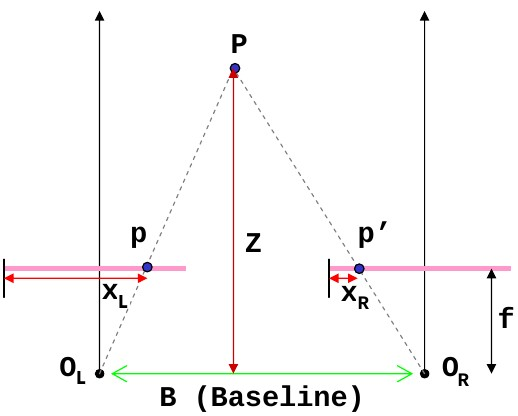
\includegraphics[width=0.8\linewidth]{./img/depth.jpg}

\begin{itemize}
\item \small{ Triangolazione}:

\begin{center}
 $\frac{B}{Z} = \frac{(B+x_{L}) - x_{R}}{Z-f}$,
$Z = \frac{B \cdot f}{x_{L} - x_{R}} = \frac{B \cdot f}{d}$
\end{center}


\item  $ d = x_{L} - x_{R} $ \`{e} la disparit\`{a} 
\end{itemize}

\end{column}
\end{columns}
\end{frame}


\begin{frame}[t]{\textsc{Corrispondenze e mappa di disparit\`{a}}}


\begin{columns}
\begin{column}{5cm}
\vspace{1em}
\begin{itemize}
\item \small{Metodi locali: calcolano un valore di similarit\`{a} (MSE, NCC..) all'interno di una finestra  
\item Metodi globali: minimizzano su tutta l'immagine una funzione di energia che racchiude le assunzioni di corrispondenza
}
\end{itemize}
\end{column}
\begin{column}{5cm}
\vspace{1.5em}
\centering
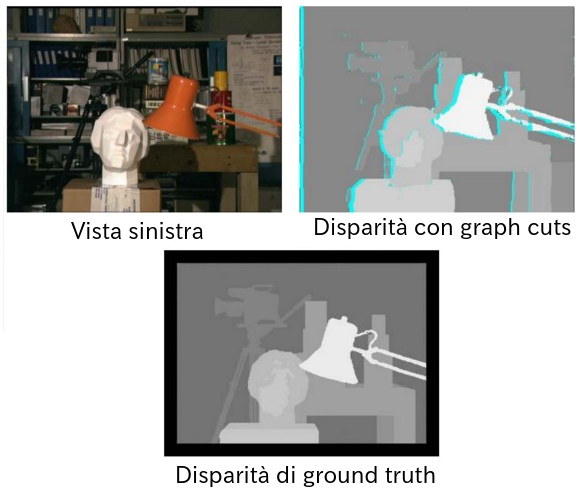
\includegraphics[width=1\linewidth]{./img/gc.png}
\end{column}
\end{columns}
\vspace{-1em}
\begin{center}
	\setbeamertemplate{blocks}[rounded][shadow=false]
	\setbeamercolor{block title}{use=structure,fg=black,bg=lightgray} 
	\setbeamercolor{block body}{use=structure,fg=black,bg=lightgray}
\begin{block}{}
\center \small{In questa tesi � stato utilizzato l'algoritmo di Kolmogorov and Zabih \textbf{Graph Cuts Stereo Matching Algorithm} per il calcolo della mappa di disparit\`{a}}
\end{block}
\end{center}
\end{frame}


\end{section}
\begin{section}{Watermarking}
\subsection {Principi del watermarking}
\begin{frame}[t]{\textsc{Watermarking}}

\end{frame}


\end{section}





\begin{section}{Metodo in frequenza}

\begin{frame}[t]{\textsc{Algoritmo di marchiatura nel dominio della frequenza}}

\begin{columns}
\begin{column}{5cm}
\begin{center}
\setbeamertemplate{blocks}[rounded][shadow=false]
%\setbeamercolor{block title}{use=structure,fg=black,bg=lightgray} 
\setbeamercolor{block body}{use=structure,fg=black,bg=lightgray} 
\begin{block}{Vantaggi:}
\center{\begin{itemize}
\item Visibilit\`{a}  e sicurezza;
\item Invariante a traslazioni, rotazioni e resizing;
\item Resistente a degradazioni;
\item Rilevazione di tipo Blind
\end{itemize}}
\end{block}
\end{center}
\end{column}
\begin{column}{5cm}
\end{column}
\end{columns}
\end{frame}


\subsection{Processo di marchiatura stereo}

\begin{frame}[t]{\textsc{Marchiatura vista sinistra}}
\begin{figure}
  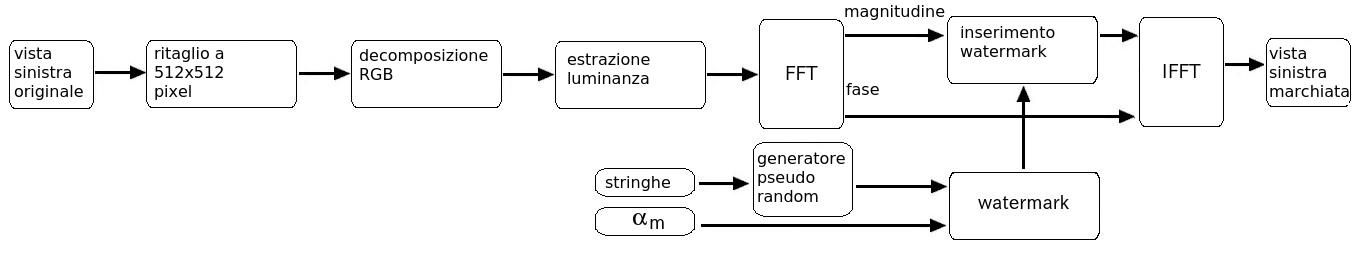
\includegraphics[width=1\textwidth]{./img_wat/left_wat.jpg}  
  \label{fig:leftwat}
\end{figure}

\begin{center}
\setbeamertemplate{blocks}[rounded][shadow=false]
%\setbeamercolor{block title}{use=structure,fg=black,bg=lightgray} 
\setbeamercolor{block body}{use=structure,fg=black,bg=lightgray} 
\begin{block}{Inserimento marchio:}
\center{\begin{itemize}
\item estrazione luminanza $Y$;
\item estrazione coefficienti a media frequeza;
\item alterazione coefficienti secondo : $y_{i} = y_{i} + \alpha w_{i} y_{i} $.
\end{itemize}}
\end{block}
\end{center}

\end{frame}



\begin{frame}[t]{\textsc{Marchiatura vista destra}}
\begin{figure}
  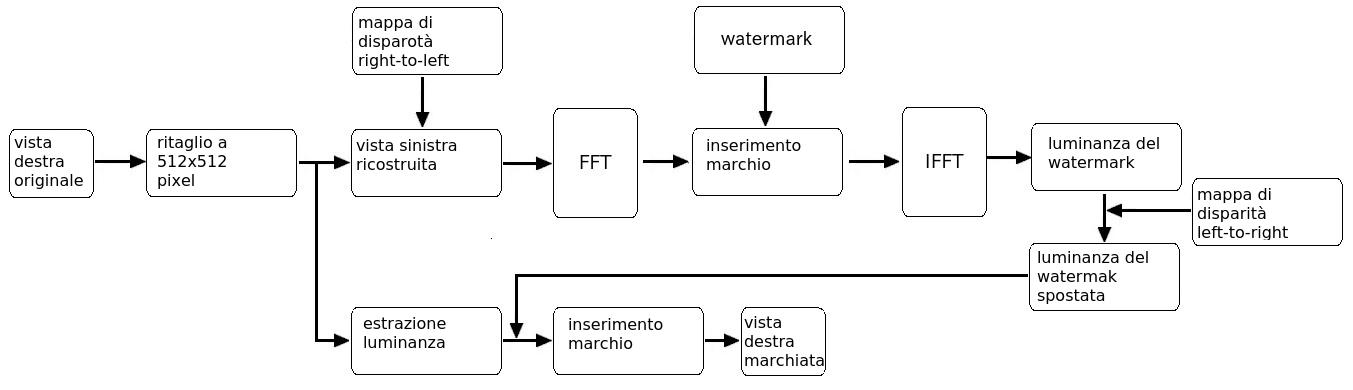
\includegraphics[width=0.95\textwidth]{./img_wat/pros.jpg}  
  \label{fig:rightwat}
\end{figure}
\setbeamertemplate{blocks}[rounded][shadow=false]
%\setbeamercolor{block title}{use=structure,fg=black,bg=lightgray} 
\setbeamercolor{block body}{use=structure,fg=black,bg=lightgray} 
\begin{block}{Obiettivi:}
\center{\begin{itemize}
\item Pixel corrispondenti marchiati nello stesso modo;
\item Marchio inserito spazialmente ma rilevabile in frequenza.
\end{itemize}}
\end{block}
\end{frame}

\begin{frame}[t]{\textsc{Marchiatura vista destra}}
Idea: 
\begin{figure}
  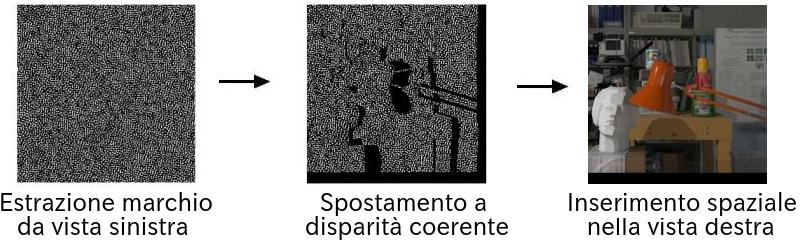
\includegraphics[width=0.75\textwidth]{./img_wat/idea.jpg}
  
  \label{fig:idea}
\end{figure}
\vspace{-3mm}
Se consideriamo l'immagine  $l$ scritta in funzione della sua trasformata  $L$ :
\begin{center}
  \scalebox{0.8}{%
$ l =  \frac{1}{MN}\sum\sum(|L(u,v)|)\exp\{\phi (u,v)\} \exp\{-j2\pi(\frac{ux}{M}\frac{vy}{N})\}  $
  }
\end{center}
Dopo il processo di marchiatura avremo: 
\begin{center}
  \scalebox{0.8}{%
$ l_{w} = \frac{1}{MN}\sum\sum(|L(u,v)| + \alpha|L(u,v)||w|)\exp\{j(\phi_{L}+\phi_{w})\}\exp\{-j2\pi(\frac{ux}{M}\frac{vy}{N})\} $
  }
\end{center}

\end{frame}

\begin{frame}[t]{\textsc{Marchiatura vista destra}}
\setbeamertemplate{blocks}[rounded][shadow=false]
%\setbeamercolor{block title}{use=structure,fg=black,bg=lightgray} 
\setbeamercolor{block body}{use=structure,fg=black,bg=lightgray} 
\begin{block}{Problemi:}
\center{\begin{itemize}
\item La procedura di detection si aspetta in ingresso un'immagine del tipo:
\begin{center}
  \scalebox{0.8}{%
$ r_{w} = r + \frac{1}{MN}\sum\sum(\alpha|R(u,v)||w|\exp\{j(\phi_{R}+\phi_{w})\})\exp\{-j2\pi(\frac{ux}{M}\frac{vy}{N})\} $
  }
\end{center}
\item L'alterazione estraibile dalla vista sinistra \`{e} del tipo:
%\vspace{-2mm}
\begin{center}
  \scalebox{0.8}{%
$ \alpha|L||w|exp\{j(\phi_{L}+\phi{w})\} $
  }
\end{center}
\end{itemize}}
\end{block}
\begin{block}{Soluzione:}
		\begin{itemize}
		\item modulo marchio: modulo della vista sinistra ricostruita a partire dai pixel della vista destra;
		\item fase marchio: fase della vista sinistra sommata a quella del marchio di riferimento; 
		\end{itemize}
\end{block}

\end{frame}


\begin{frame}[t]{\textsc{Marchiatura vista destra}}
\vspace{5mm}
Il marchio inserito nella vista destra \`{e} quindi:
\begin{center}
  \scalebox{1}{%
$ \alpha|R^{**}||w|exp\{j(\phi_{L}+\phi{w})\} $
  }
\end{center}
\vspace{3mm}
Le formule complete sono:
\vspace{3mm}
\begin{center}
  \scalebox{0.9}{%
$ l_{w} = l + \frac{1}{MN}\sum\sum(\alpha|L(u,v)||w|\exp\{j(\phi_{L}+\phi_{w})\})\exp\{-j2\pi(\frac{ux}{M}\frac{vy}{N})\} $

  }
\end{center}
\begin{center}
  \scalebox{0.9}{%

$ r_{w} = r + \frac{1}{MN}\sum\sum(\alpha|R(u,v)^{**}||w|\exp\{j(\phi_{L}+\phi_{w})\})^{*}\exp\{-j2\pi(\frac{ux}{M}\frac{vy}{N})\} $
  }
\end{center}
\end{frame}


\begin{frame}[t]{\textsc{Detection vista sinistra}}

\begin{figure}
  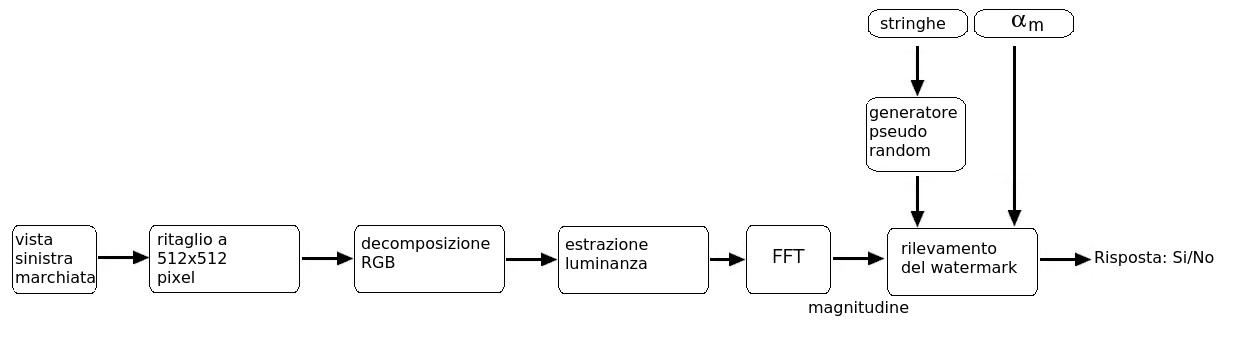
\includegraphics[width=0.95\textwidth]{./img_wat/left_det.jpg}
  
  \label{fig:leftdet}
\end{figure}
\setbeamertemplate{blocks}[rounded][shadow=false]
%\setbeamercolor{block title}{use=structure,fg=black,bg=lightgray} 
\setbeamercolor{block body}{use=structure,fg=black,bg=lightgray} 
\begin{block}{Detection basata su soglia:}
\center{\begin{itemize}
\item generazione marchio;
\item calcolo likelihood $L(y)$ e soglia $\lambda$ con il criterio di Neyman-Pearson;
\item comparazione $L(y)$ con $\lambda$ e decisione.
\end{itemize}}
\end{block}
\end{frame}

\begin{frame}[t]{\textsc{Detection vista destra}}
\begin{figure}
  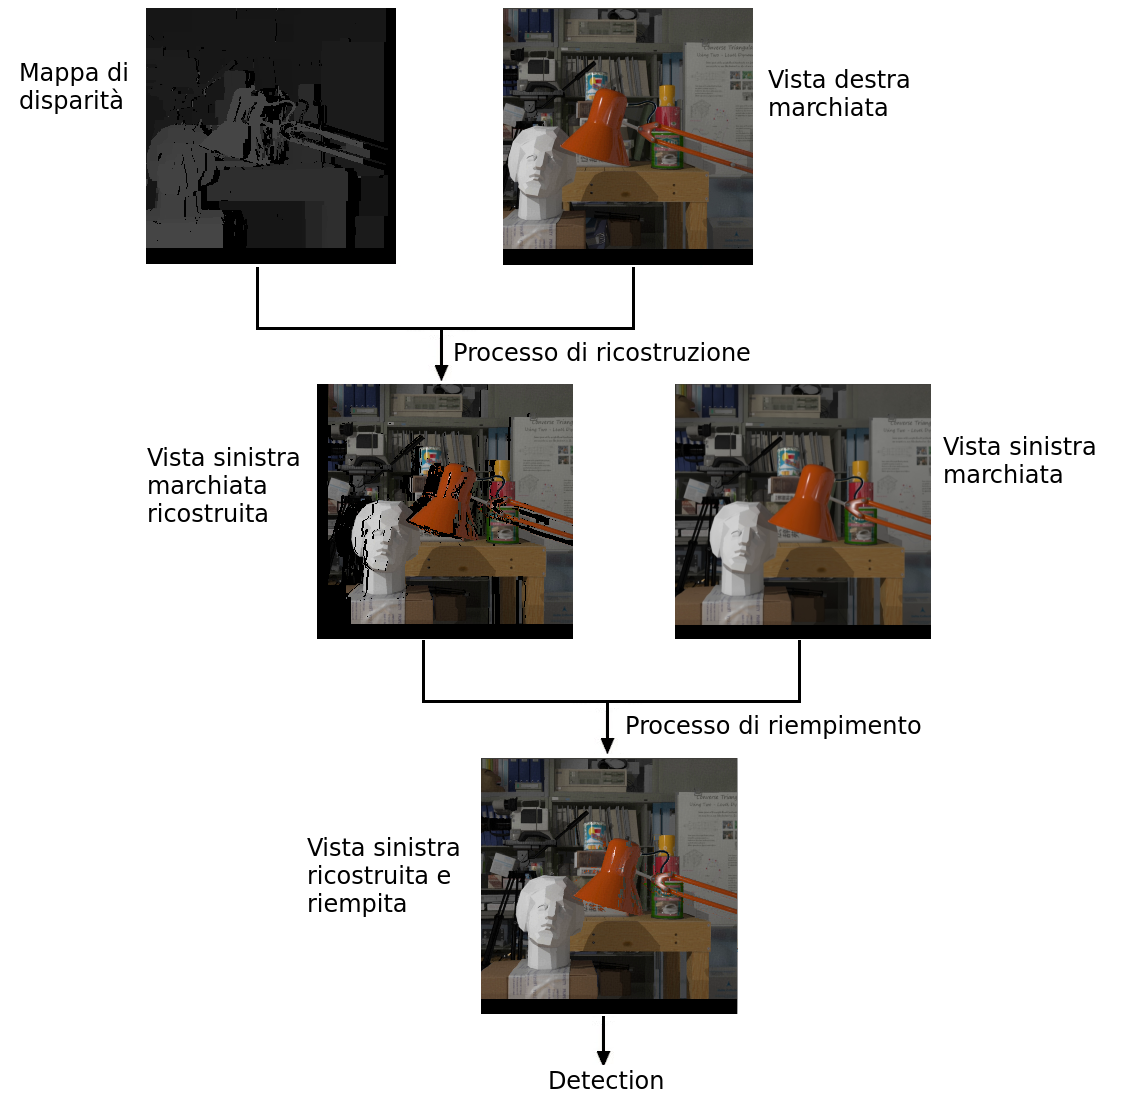
\includegraphics[width=0.65\textwidth]{./img_wat/detection_workflow.png}  
  \label{fig:rightdetflow}
\end{figure}
\end{frame}

\end{section}

\begin{section}{Risultati sperimentali}

\begin{frame}[t]{\textsc{Risultati sperimentali}}
Test effettuati su:
\begin{itemize}
\item sequenza video di 1 minuto creata dal dataset Tsukuba
\item frame rate 30
\item group of picture 60
\end{itemize}

\vspace{2mm}
\begin{figure}
  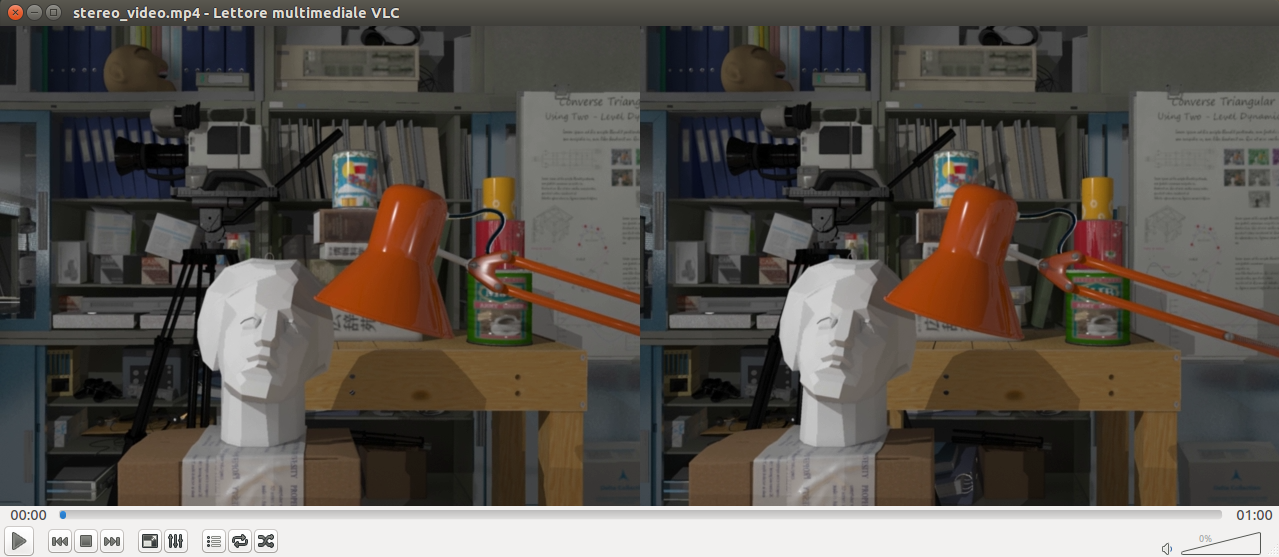
\includegraphics[width=0.8\textwidth]{./img_wat/video_stereo.png}  
  \label{fig:video}
\end{figure}
\end{frame}

\subsection{Risultati sperimentali}

\begin{frame}[t]{\textsc{Test di robustezza}}
\setbeamertemplate{blocks}[rounded][shadow=false]
%\setbeamercolor{block title}{use=structure,fg=black,bg=lightgray} 
\setbeamercolor{block body}{use=structure,fg=black,bg=lightgray} 
\begin{block}{Compressione:}
Si studia la degradazione del marchio dovuta alla compressione del video, in relazione alla potenza di inserimento.
\end{block}
\begin{block}{Distribuzione web:}
Si studia la resistenza del marchio in video che sono stati caricati su Youtube e successivamente scaricati.
\end{block}
\begin{block}{Sintetizzazione di viste intermedie:}
Si studia la risposta del marchio in caso di creazione di viste sintetiche a tre diverse distanze dalla vista sinistra.
\end{block}

\end{frame}

\begin{frame}[t]{\textsc{Compressione}}
\vspace{-2mm}
\begin{table}
\scalebox{0.6}{
\begin{tabular}{c | c | c }
potenza marchio & livello di compressione & Detection stereo \\
\hline \hline
\rowcolor{LRed}  \textbf{1} & \textbf{1} & \textbf{80\%} \\
1 & 15 & 40\%\\
 1 & 25 & $< 20\% $\\
 1 & 30 & $< 20\% $ \\\hline
 3 & 1 &  $ >90\% $\\
3 & 15 &  $ >90\% $\\
 3 & 25 & $ >90\% $\\
 3 & 30 &  $ >90\% $ \\\hline

\end{tabular}
}

\end{table}
\begin{center}
\scalebox{0.7}{Statistica della detection spaziale}
\end{center}
\vspace{-2mm}
\begin{table}
\scalebox{0.6}{
\begin{tabular}{c | c | c }
potenza marchio & livello di compressione & Detection stereo \\
\hline \hline
 0.3 & 1 & 100\% \\
\rowcolor{LRed} \textbf{0.3} & \textbf{15} & \textbf{$ >96\% $}\\
 0.3 & 25 & 36.6\%  \\
 0.3 & 30 & 6.6\% \\\hline
 0.6 & 1 & 100\%  \\
 0.6 & 15 & 100\%  \\
\rowcolor{LRed} \textbf{0.6} & \textbf{25} & 86.6\% \\
 0.6 & 30 & 50\% \\
\end{tabular}
}
\end{table}
\begin{center}
\scalebox{0.7}{Statistica della detection in frequenza}
\end{center}
\end{frame}



\begin{frame}[t]{\textsc{Distribuzione web}}
\begin{table}
\scalebox{0.75}{
\begin{tabular}{c | c }
potenza del marchio & Detection stereo \\
\hline \hline
0.3 & 1 \\
0.5 & 6 \\
0.6 & 11\\
\end{tabular}
}
\vspace{2mm}
\caption{Statistica della detection in frequenza per video caricati su Youtube}
\end{table}
Analisi PSNR:
\begin{table}
\scalebox{0.75}{
\begin{tabular}{c | c }
livello di compressione & PSNR \\
\hline \hline
15 		    & 46.0194 \\
25 		    & 40.4861 \\
YT 		    & 38.2039 \\
30 		    & 37.5587 \\
\end{tabular}
}
\vspace{2mm}
\caption{Valore medio di PSNR per diversi livelli di compressione}
\end{table}
\end{frame}
\begin{frame}[t]{\textsc{Sintetizzazione di viste intermedie}}

\begin{figure}
\vspace{1mm}
  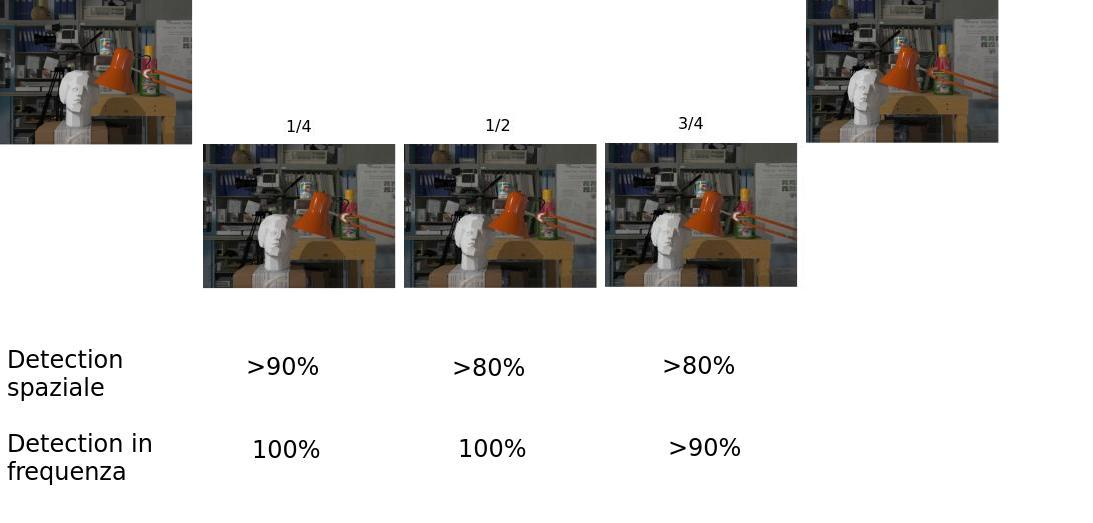
\includegraphics[width=1.1\textwidth]{./img_wat/synt.jpg}  
  \caption{} 
  \label{fig:vsg1}
\end{figure}


\end{frame}



\begin{frame}[t]{\textsc{Test di invisibilit\`{a}: misure di qualit\`{a} }}
\vspace{-13mm}
\begin{columns}
\begin{column}{5cm}
\begin{center}
\vspace{10mm}
\begin{figure}
  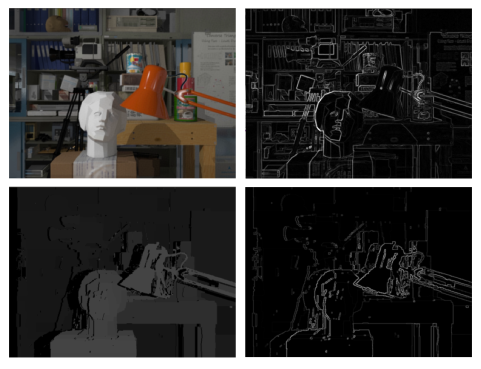
\includegraphics[width=1\textwidth]{./img_wat/quality.png}  
  \caption{} 
  \label{fig:qm}
\end{figure}
\end{center}
\end{column}
\begin{column}{5cm}
\vspace{-17mm}
\begin{center}
  \scalebox{0.65}{%
$ Q_{View}(x,y) = [l(x,y)]^{\alpha} \cdot [c(x,y)]^{\beta} \cdot [\mathbf{{S}_{View}(x',y')]^{\gamma}} $
  }
\end{center}

\vspace{2mm}

\begin{center}
  \scalebox{0.65}{%
$ Q_{Depth}(x,y) = [l(x,y)]^{\alpha} \cdot [c(x,y)]^{\beta} \cdot [\mathbf{{S}_{Depth}(x',y')]^{\gamma}} $
  }
\end{center}

\end{column}

\end{columns}
\vspace{-7mm}
\setbeamertemplate{blocks}[rounded][shadow=false]
%\setbeamercolor{block title}{use=structure,fg=black,bg=lightgray} 
\setbeamercolor{block body}{use=structure,fg=black,bg=lightgray} 

\begin{block}{\small Metriche di Chamida et al.}
\begin{itemize}
\item \small Basate sugli \textbf{edge} della mappa di disparit\`{a} e della vista da esaminare
\item \small Versione modificata di \textbf{SSIM} 
\item \small Metrica di tipo \textbf{Reduced-Reference} 
\end{itemize}
\end{block}
\end{frame}


\begin{frame}[t]{\textsc{Test di invisibilit\`{a}: misure di qualit\`{a} }}
\vspace{-3mm}
\begin{figure}
  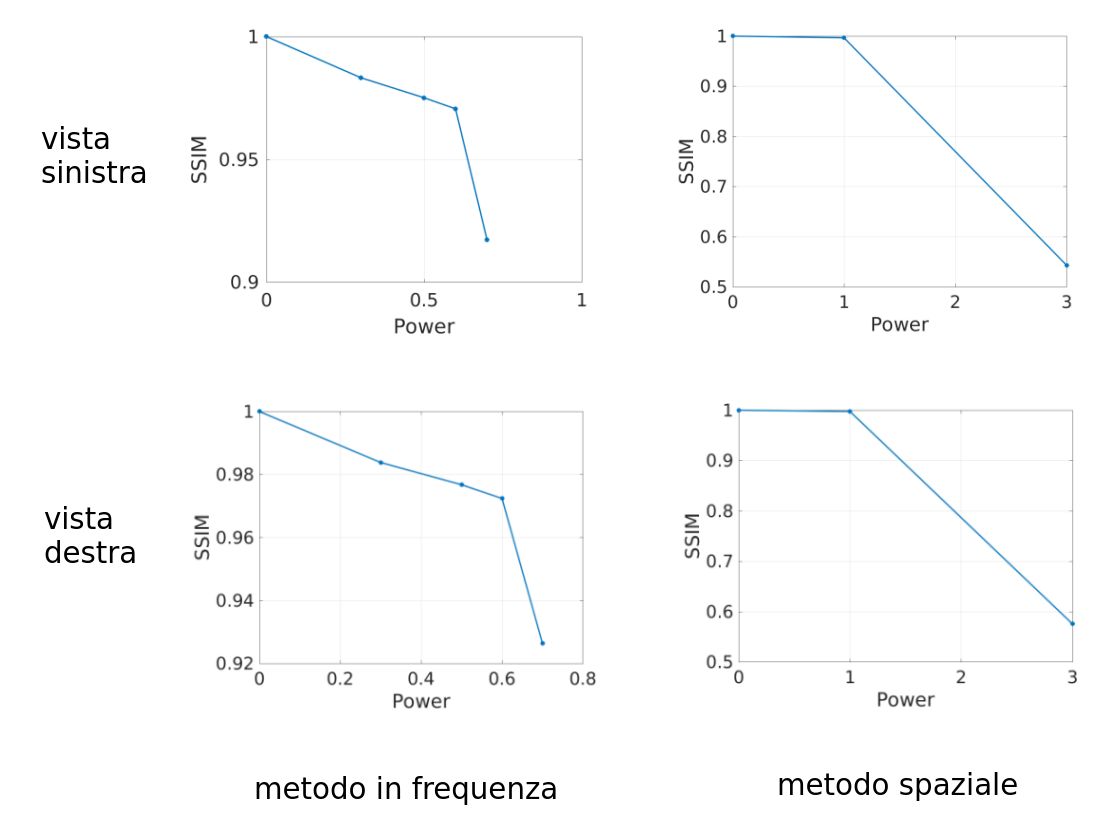
\includegraphics[width=0.9\textwidth]{./img_wat/qm_res.png}  
  \caption{} 
  \label{fig:qmgr}
\end{figure}


\end{frame}

\begin{frame}[t]{\textsc{Test di invisibilit\`{a}: PSNR}}
\setbeamertemplate{blocks}[rounded][shadow=false]
\setbeamercolor{block title}{use=structure,fg=black,bg=lightgray} 
\setbeamercolor{block body}{use=structure,fg=black,bg=lightgray} 
\begin{block}{}

\begin{itemize}
\item Si \`{e} misurato l'impatto visivo tramite PSNR tra i frame originali e marchiati;
\item valori tipici per video marchiati sono tra 30 e 50 dB.
\end{itemize}
\end{block}

\begin{table}
\scalebox{0.8}{
\begin{tabular}{c | c }
potenza del marchio & PSNR(dB) \\
\hline \hline
0.3 		    & 46.0071 \\
0.5		    & 45.9505 \\
0.6		    & 45.9291 \\
\end{tabular}
}
\vspace{2mm}
\caption{Valore medio di PSNR al variare della potenza del marchio}
\end{table}
\end{frame}

\end{section}

\begin{section}{Conclusioni}
\subsection{Conclusioni}


\begin{frame}[t]{\textsc{Conclusioni}}
Nel dominio spaziale:
\begin{columns}
\begin{column}{5cm}
\setbeamertemplate{blocks}[rounded][shadow=false]
\setbeamercolor{block title}{use=structure,fg=black,bg=lightgray} 
\setbeamercolor{block body}{use=structure,fg=black,bg=lightgray} 
\begin{block}{}
\begin{itemize}
\item fissiamo un degrado della qualit\`{a} dell'immagine del 1\%
\item otteniamo la potenza del marchio pari a 1
\end{itemize}
\end{block}
\end{column}

\begin{column}{5cm}
\vspace{-6mm}
\begin{table}
\scalebox{0.65}{
\begin{tabular}{c | c | c }
CRF & potenza del marchio & True positive \\
\hline \hline
\rowcolor{LRed} 1 & 1 & 70\%\\
15 & 1 & 40\%\\
25 & 1 & $< 20\% $\\
30 & 1 & $< 20\% $\\
\end{tabular}
}
\end{table}

\end{column}
\end{columns}
\vspace{2mm}
\begin{figure}
  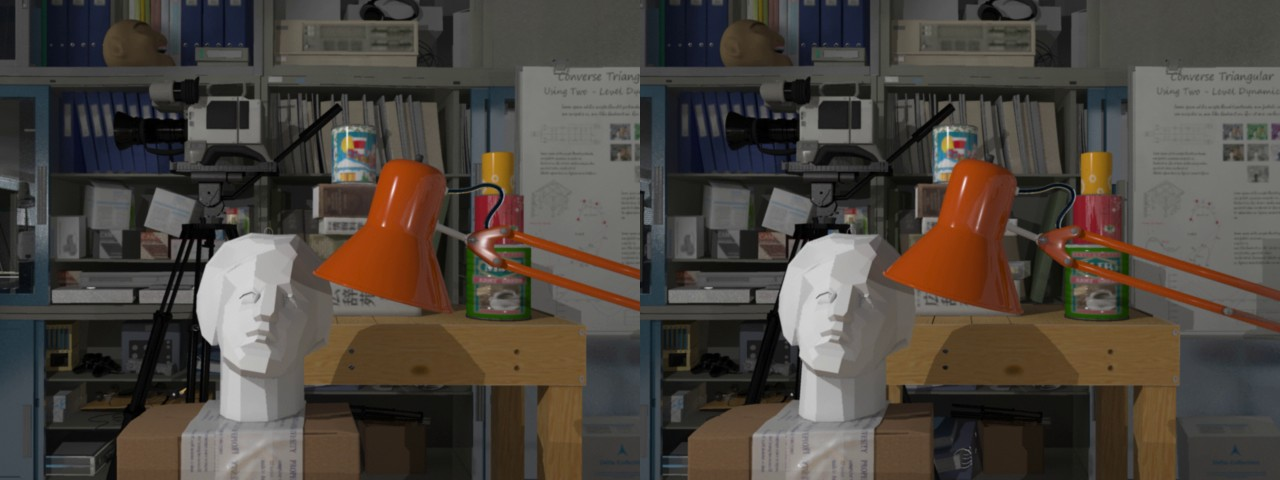
\includegraphics[width=0.7\textwidth]{./img_wat/marked_1_gauss.jpg}  
  \caption{} 
  \label{fig:mg1}
\end{figure}
\end{frame}


\begin{frame}[t]{\textsc{Conclusioni}}
Nel dominio della frequenza:
\begin{columns}
\begin{column}{5cm}
\setbeamertemplate{blocks}[rounded][shadow=false]
\setbeamercolor{block title}{use=structure,fg=black,bg=lightgray} 
\setbeamercolor{block body}{use=structure,fg=black,bg=lightgray} 
\begin{block}{}
\begin{itemize}
\item fissiamo un degrado della qualit\`{a} dell'immagine del 1\%
\item otteniamo la potenza del marchio pari a 0.3 
\end{itemize}
\end{block}

\end{column}
\begin{column}{5cm}
\vspace{-10mm}
\begin{table}
\scalebox{0.65}{
\begin{tabular}{c | c | c }
CRF & potenza del marchio & detection stereo \\
\hline \hline
1 & 0.3 & 100\%\\
\rowcolor{LRed} 15 & 0.3 & $>90\%$\\
25 & 0.3 & 36.6\%\\
30 & 0.3 & 6.6\%\\
\end{tabular}
}
\end{table}

\end{column}
\end{columns}
\vspace{2mm}
\begin{figure}
  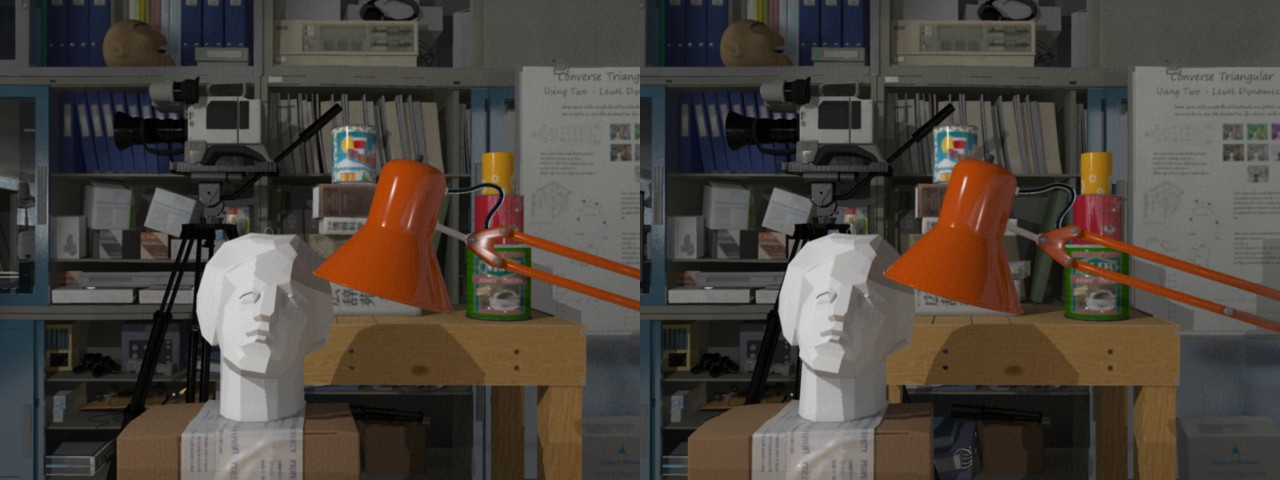
\includegraphics[width=0.7\textwidth]{./img_wat/marked_03_DFT.jpg}  
  \caption{} 
  \label{fig:mg1}
\end{figure}
\end{frame}

\begin{frame}[t]{\textsc{Conclusioni}}
Video stereo marchiato con potenza 0.3 compresso a fattore 15
\vspace{2mm}
\begin{center}
\movie[width=8cm,height=6cm,autostart,loop,poster]{}{./img_wat/anaglifico_03_kz.mkv}
\end{center}

\end{frame}
\end{section}



\end{document}
